% \begin{figure}[!ht]
% 	\centering
% 	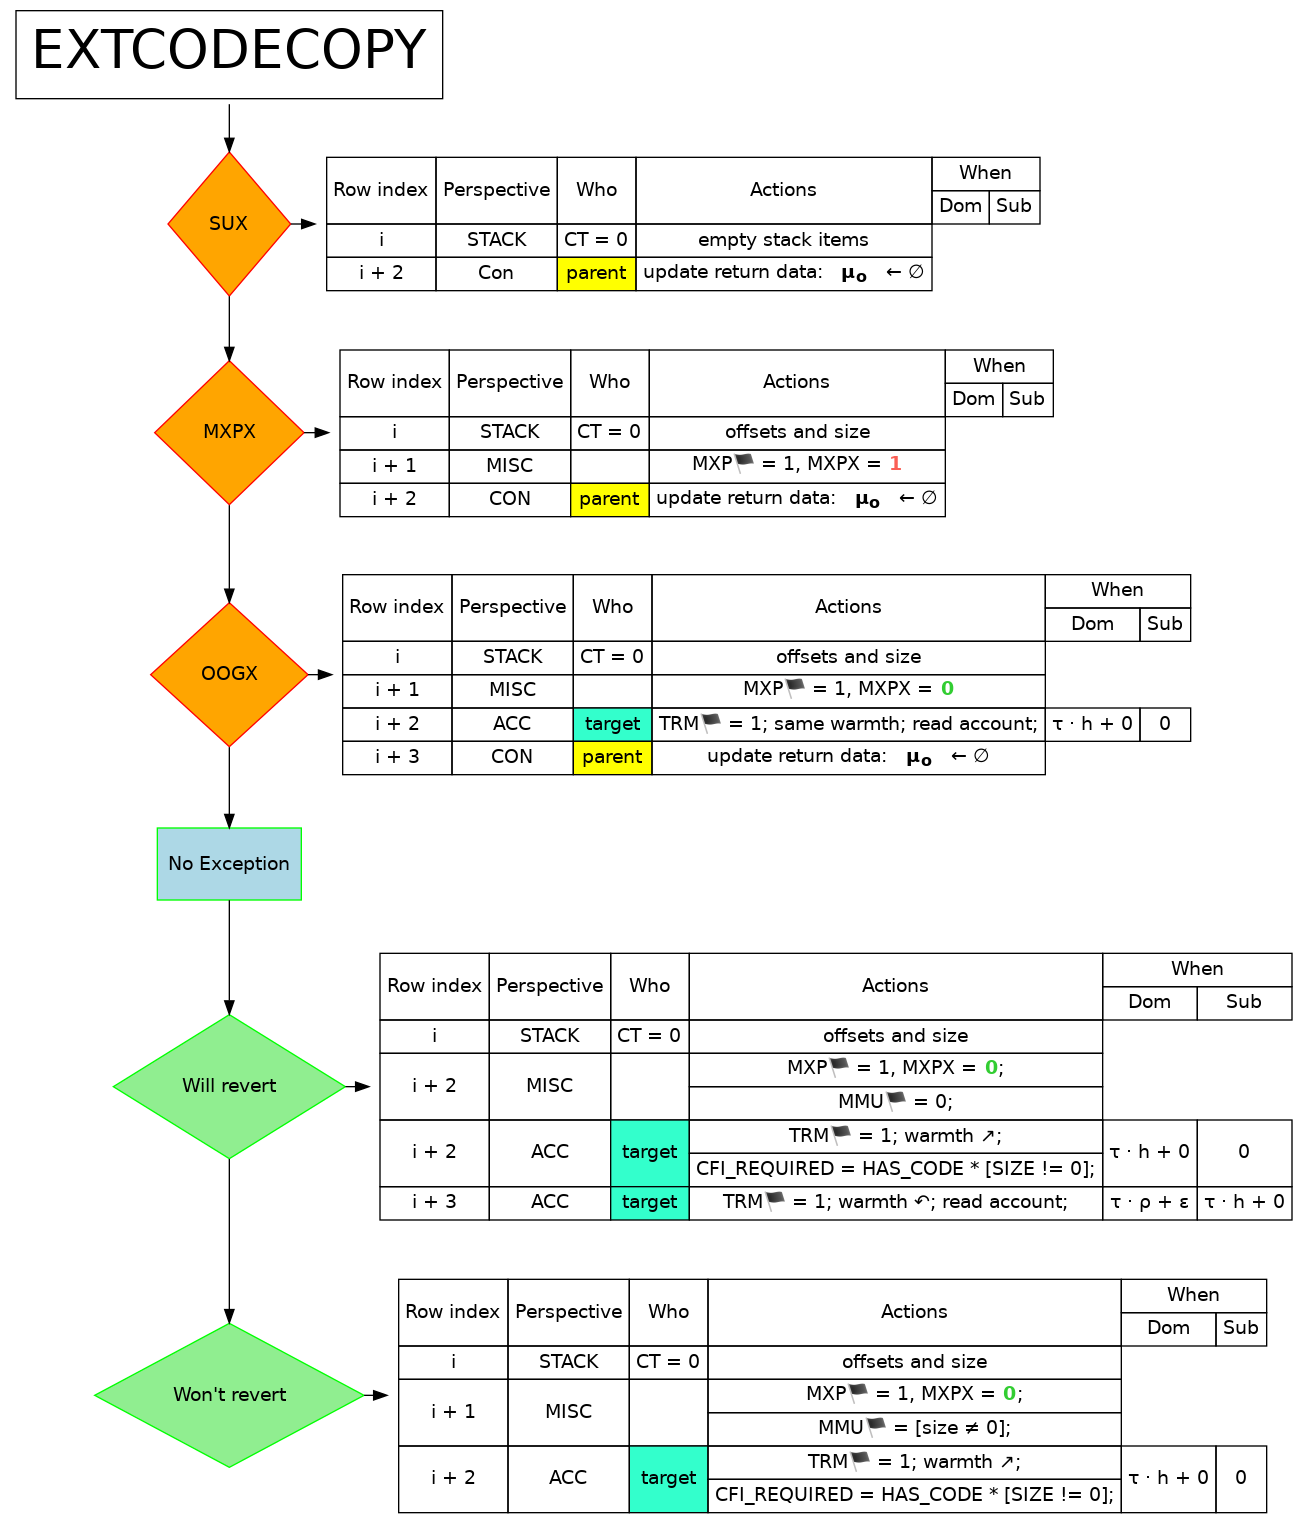
\includegraphics[width=\textwidth]{instruction_handling/copy/flowcharts/extcc.png}
% 	\caption{General workflow for \inst{EXTCODECOPY} instructions. We use the abbreviation $\rho := \cnRevStamp_{i}$.}
% 	\label{fig: hub: instruction handling: copy: extcodecopy: general processing}
% \end{figure}

\begin{center}
	\boxed{%
		\text{The stack constraints presented below assume }
		\left\{ \begin{array}{lcl}
			\peekStack        _{i}                  & = & 1 \\
			\stackDecCopyFlag _{i}                  & = & 1 \\
			\locIsExtcc                             & = & 1 \\
			\stackSux         _{i} + \stackSox _{i} & = & 0 \\
		\end{array} \right.}
\end{center}
The \inst{EXTCODECOPY} instruction is the most complex of all instructions in the \inst{COPY} instruction family.
Indeed it \emph{may} require any of the following
(\emph{a}) trimming of the address argument
(\emph{b}) loading bytecode into the \romMod{}
(\emph{c}) considering whether the target address is undoing deployment or not
(\emph{d}) turning on the target account's warmth
(\emph{e}) and, in case of an upcoming revert, undoing the previous turning on of the target account's warmth.
Recall that depending on whether the instruction produces an \mxpxSH{} or not we either peek into the caller context (and provide it with empty return data)
or inspect the called account. The specialized constraints are as follows.
\begin{description}
		% - [x] context stuff,
		% - [x] gas cost stuff,
		% - [ ] account stuff,
		% - [x] trimming stuff,
		% - [x] cfi stuff,
		% - [ ] setting and unsetting warmth,
		% - [ ] account remain unchanged otherwise,
		% - [∅] etc ...
	\item[\underline{\underline{Setting the gas cost:}}]
		we only set the gas cost to the actual gas cost if no \mxpxSH{} has occurred (given no stack exception, that is):
		\begin{enumerate}
			\item \If $\stackMxpx _{i} = 1$ \Then $\gasCost_{i} = 0$
			\item \If $\stackMxpx _{i} = 0$ \Then 
				\[ 
				\gasCost_{i}
				=
				\left[ \begin{array}{cl}
					+ & \stackStaticGas_{i} \\
					+ & \locMxpGas     \\
					+ & \left[\begin{array}{crcl}
						+ & \locAddressIsWarm       & \cdot & G_\text{warmaccess}        \\
						+ & (1 - \locAddressIsWarm) & \cdot & G_\text{coldaccountaccess} \\
					\end{array} \right] \\
				\end{array} \right]
				\]
		\end{enumerate}
	\item[\underline{\underline{The \mxpxSH{} case:}}]
		\If $\stackMxpx_{i} = 1$ \Then
		\[
			\executionProvidesEmptyReturnData {i}{\locCopyCallerContextRowSmall}
		\]
	\item[\underline{\underline{The \oogxSH{} case:}}]
		\If $\stackOogx _{i} = 1$ \Then
		we impose the following:
		\begin{description}
			\item[\underline{Setting the account row $n^°(i + \locCopyOutsideAccountRowFirst)$:}] 
				we impose that
				\[
					\left\{ \begin{array}{lclr}
						\multicolumn{4}{l}{\accTrimAddress
						{i}{\locCopyOutsideAccountRowFirst}
						{\locAddressParamHi}
						{\locAddressParamLo}} \\
						\accRomLexFlag  _{i + \locCopyOutsideAccountRowFirst} & = & \rZero \\
						\multicolumn{4}{l}{\accSameBalance                    {i}{\locCopyOutsideAccountRowFirst}}    \\
						\multicolumn{4}{l}{\accSameNonce                      {i}{\locCopyOutsideAccountRowFirst}}    \\
						\multicolumn{4}{l}{\accSameCode                       {i}{\locCopyOutsideAccountRowFirst}}    \\
						\multicolumn{4}{l}{\accSameDeployment                 {i}{\locCopyOutsideAccountRowFirst}}    \\
						\multicolumn{4}{l}{\accSameWarmth                     {i}{\locCopyOutsideAccountRowFirst}}    \\
						\multicolumn{4}{l}{\accSameMarkedForSelfdestructFlag  {i}{\locCopyOutsideAccountRowFirst}}    \\
						\multicolumn{4}{l}{
							\standardDomSubStamps {
								anchorRow        = i,
								relOffset        = \locCopyOutsideAccountRowFirst,
								domOffset        = 0,
							}
						} \\
					\end{array} \right.
				\]
			\item[\underline{Setting the context row $n^°(i + \locCopyCallerContextRowLarge )$:}] 
				we impose that
				\[
					\executionProvidesEmptyReturnData {i}{\locCopyCallerContextRowLarge}
				\]
		\end{description}
	\item[\underline{\underline{Specifying \locTriggerCfi{}:}}]
		\inst{EXTCODECOPY} is the only instruction in the \inst{COPY}-family that \textbf{may} require loading (new) bytecode into the \romMod{} module;
		this is required precisely for \textbf{unexceptional} executions that copy a \textbf{nonzero} number of bytes from an address with \textbf{nonempty bytecode};
		as such we impose:
		\[
			\locTriggerCfi = \locIsExtcc \cdot \locTriggerMmu \cdot \locHasCode
		\]
		\saNote{} By construction the \locTriggerMmu{} flag, see section~(\ref{locTriggerMmu for the copy family}), \locTriggerMmu{} is off whenever an exception occurs or the instruction is unexceptional but has zero size.
	\item[\underline{\underline{The unexceptional, reverted case:}}]
		\If $\xAhoy_{i} = 0$ \et $\cnWillRev_{i} = 1$ \Then 
		\begin{description}
			\item[\underline{The ``doing''   account-row $n^°(i + \locCopyOutsideAccountRowFirst )$:}] 
				we impose that
				\[
					\left\{ \begin{array}{lclr}
						\multicolumn{4}{l}{\accTrimAddress
						{i}{\locCopyOutsideAccountRowFirst}
						{\locAddressParamHi}
						{\locAddressParamLo}} \\
						\accRomLexFlag    _{i + 2} & = & \locTriggerCfi   \vspace{2mm} \\
						\multicolumn{4}{l}{\accSameBalance                    {i}{\locCopyOutsideAccountRowFirst}}    \\
						\multicolumn{4}{l}{\accSameNonce                      {i}{\locCopyOutsideAccountRowFirst}}    \\
						\multicolumn{4}{l}{\accSameCode                       {i}{\locCopyOutsideAccountRowFirst}}    \\
						\multicolumn{4}{l}{\accSameDeployment                 {i}{\locCopyOutsideAccountRowFirst}}    \\
						\multicolumn{4}{l}{\accTurnOnWarmth                   {i}{\locCopyOutsideAccountRowFirst}}    \\
						\multicolumn{4}{l}{\accSameMarkedForSelfdestructFlag  {i}{\locCopyOutsideAccountRowFirst}}    \\
						\multicolumn{4}{l}{
							\standardDomSubStamps {
								anchorRow        = i,
								relOffset        = \locCopyOutsideAccountRowFirst,
								domOffset        = 0,
							}
						} \\
							% \standardDomSubStamps              {i}{\locCopyOutsideAccountRowFirst}{0}} \\
					\end{array} \right.
				\]
			\item[\underline{The ``undoing'' account-row $n^°(i + \locCopyOutsideAccountRowSecond )$:}] 
				we impose that
				\[
					\left\{ \begin{array}{lclr}
						\multicolumn{4}{l}{\accSameAddr                            {i}{\locCopyOutsideAccountRowSecond}{\locCopyOutsideAccountRowFirst}} \\
						\accRomLexFlag  _{i + \locCopyOutsideAccountRowSecond} & = & 0  & (\trash) \vspace{2mm} \\
						\multicolumn{4}{l}{\accUndoBalanceUpdate                   {i}{\locCopyOutsideAccountRowSecond}{\locCopyOutsideAccountRowFirst}} \\
						\multicolumn{4}{l}{\accUndoNonceUpdate                     {i}{\locCopyOutsideAccountRowSecond}{\locCopyOutsideAccountRowFirst}} \\
						\multicolumn{4}{l}{\accUndoCodeUpdate                      {i}{\locCopyOutsideAccountRowSecond}{\locCopyOutsideAccountRowFirst}} \\
						\multicolumn{4}{l}{\accUndoDeploymentStatusAndNumberUpdate {i}{\locCopyOutsideAccountRowSecond}{\locCopyOutsideAccountRowFirst}} \\
						\multicolumn{4}{l}{\accUndoWarmthUpdate                    {i}{\locCopyOutsideAccountRowSecond}{\locCopyOutsideAccountRowFirst}} \\
						\multicolumn{4}{l}{\accSameMarkedForSelfdestructFlag       {i}{\locCopyOutsideAccountRowSecond}}                                 \\
						\multicolumn{4}{l}{
							\revertDomSubStamps {
								anchorRow        = i,
								relOffset        = \locCopyOutsideAccountRowSecond,
								subOffset        = 1,
							}
						} \\
							% {i}{\locCopyOutsideAccountRowSecond}{1}}
					\end{array} \right.
				\]
		\end{description}
		\saNote{} With the the first constraints we impose a lookup to the \trmMod{} module (and hence the correction of the ``address parameter'' of \inst{EXTCODECOPY}.)
		With the second constraints we impose a lookup to the \romLexMod{} (and hence get access to the relevant \CFI{}.) 
	\item[\underline{\underline{The unexceptional, unreverted case:}}]
		\If $\xAhoy_{i} = 0$ \et $\cnWillRev_{i} = 0$ \Then 
		\[
			\left\{ \begin{array}{lclr}
				\multicolumn{4}{l}{\accTrimAddress
				{i}{\locCopyOutsideAccountRowFirst}
				{\locAddressParamHi}
				{\locAddressParamLo}} \\
				\accRomLexFlag  _{i + \locCopyOutsideAccountRowFirst}                                          & = & \locTriggerCfi   \vspace{2mm} \\
				\multicolumn{4}{l}{\accSameBalance                    {i}{\locCopyOutsideAccountRowFirst}}    \\
				\multicolumn{4}{l}{\accSameNonce                      {i}{\locCopyOutsideAccountRowFirst}}    \\
				\multicolumn{4}{l}{\accSameCode                       {i}{\locCopyOutsideAccountRowFirst}}    \\
				\multicolumn{4}{l}{\accSameDeployment                 {i}{\locCopyOutsideAccountRowFirst}}    \\
				\multicolumn{4}{l}{\accTurnOnWarmth                   {i}{\locCopyOutsideAccountRowFirst}}    \\
				\multicolumn{4}{l}{\accSameMarkedForSelfdestructFlag  {i}{\locCopyOutsideAccountRowFirst}}    \\
				\multicolumn{4}{l}{
					\standardDomSubStamps {
						anchorRow        = i,
						relOffset        = \locCopyOutsideAccountRowFirst,
						domOffset        = 0,
					}
				} \\
					% \standardDomSubStamps              {i}{\locCopyOutsideAccountRowFirst}{0}} \\
			\end{array} \right.
		\]
\end{description}
